

\section{Прореживание (децимация) стационарного процесса}

\textbf{Автор:} Шамсутдинов Альберт Маратович, Б-01-001	

\subsection{Основные понятия}
\subsubsection{Определение случайного процесса}
\label{sec:def}
Понятие \textsl{случайного процесса} может быть рассмотрено с двух различных, хотя близких по смыслу, сторон.

C одной стороны, пусть $(\Omega, \mathscr{A}, \mathbb{P})$ - некоторое вероятностное пространство, где $\Omega$ - пространство элементарных событий, $\mathscr{A}$ - $\sigma-$алгебра, $\mathbb{P}$ - вероятностная мера, и $T \subseteq  \mathbb{R}$. Будем называть $T$ \textsl{областью определения} процесса. Под \textsl{случайным процессом} $X$ онимают некоторое семейство случайных величин $\{x(t)\}_{t \in T}$, определённых на одном
и том же вероятностном пространстве $(\Omega, \mathscr{A}, \mathbb{P})$. Индексирующий параметр $t \in T$ часто интерпретируют как \textsl{время}. Мы будем рассматривать лишь случайные процессы, принимающие значения в измеримом пространстве $(\mathbb{R}, \mathscr{B}(\mathbb{R}))$, так что  для любого $t \in T$ $x(t):\Omega \to \mathscr{X}$, где $\mathscr{X} \subseteq \mathbb{R}$ - множество возможных значений процесса $X$. Стоит заметить, что случайный процесс является семейством функций двух аргументов: $X = \{x(\omega, t)\}_{\omega \in \Omega, t \in T}$. Аргумент $\omega$ является элементарным событием и принадлежит пространству элементарных событий $\Omega$ с заданной на нем вероятностной мерой. При фиксированном $\omega \in \Omega$ $x(t)$ можно
рассматривать как функцию переменной $t$ называемую \textsl{траекторией} или \textsl{выборочным значением} процесса. Множество всех траекторий называется \textsl{ансамблем}. В каждое время $t_{0}$ и для каждого $\omega_{0} \in \Omega$ у нас имеется число $x(t_{0}, \omega_{0})$. Для
различных $\omega_{i} \in \Omega$ в фиксированный момент времени $t_{0}$ числа $x(t_{0}, \omega_{i})$ представляют собой случайную величину, обозначаемую $X(t_0)$. В конце концов, случайная величина - это не что иное, как присвоение действительных чисел результатам случайного эксперимента. Это очень важное наблюдение и мост, соединяющий концепцию случайного процесса с более привычной концепцией случайной величины. Другими словами, в любой момент времени значение случайного процесса представляет собой случайную величину.


\begin{figure}[b]
\centering
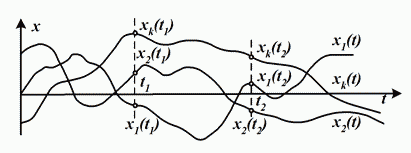
\includegraphics[width=0.8\linewidth]{kekmek1_pic_1.png}
\caption{Реализация случайного процесса $X(t)$}
\label{fig:X}
\end{figure}

Дадим альтернативное определение, рассматривающее случайный процесс как измеримое отображение из вероятностного пространство на пространство траекторий. В такой формулировке процесс выступает в качестве \textsl{случайной функции} от аргумента $t \in T$. Если $T$ — дискретно, то $X$ называют процессом с дискретным временем. Если $T$ — непрерывно, то, соответственно, $X$ называется процессом с непрерывным временем. Этот второй взгляд на случайные процессы, хотя и менее интуитивный, более подходит для точного математического развития теории случайных процессов.
\newpage
\subsubsection{Понятие стационарного процесса}

%\textbf{Определение.} $X$ называется \textsl{стационарным в узком смысле}, если его конечномерные %распределения инвариантны относительно сдвига времени, т.е. для любых $t_1,\dots,t_n \in T$ и $B \in %\mathscr{B(\mathbb{R})}^{n}$:
%{\centering $\mathbb{P}_{t_1,\dots,t_n}(B) = \mathbb{P}_{t_1 + h,\dots,t_n+h}(B)$ \par}

\begin{definition} $X$ называется \textsl{стационарным в широком смысле} процессом, если $\mathbb{E}|X(t)|^{2} < \infty$ для любого $t \in T$ и его среднее и ковариация инвариантны относительно сдвига по времени, т.е. для любых $t, s \in T$:

{\centering 
\begin{equation}
\left\{
    \begin{array}{lr}
        \mathbb{E}(X(t)) = \mathbb{E}(X(t+h)) \\
         Cov(X(t), X(s)) =  Cov(X(t+h), X(s+h))
    \end{array} 
\right.
\end{equation}
}
\end{definition}

\subsubsection{Мощность и энергия}
Благодаря определению случайного процесса, данного в~\ref{sec:def}, мы можем определить понятие мощности и энергии случайного процесса. Пусть $X(t)$-случайный процесс с произвольным выборочным значением $x(t, \omega_{i})$. Тогда энергия и мощность каждой такой функции определено следующим образом:

{\centering 
$$\mathcal{E}_{i} = \int\limits_{-\infty}^{+\infty} x^2(t, \omega_i) dt$$ \\
$$\mathcal{P}_i = \lim\limits_{T\to\infty} \frac{1}{T} \int\limits_{-\frac{T}{2}}^{\frac{T}{2}} x^2(t, \omega_i) dt$$
\par}

Соотношения показывают, что для каждого $\omega_i \in \Omega$ существуют действительные числа 
$\mathcal{E}_i$ и $\mathcal{P}_i$, характеризующий энергию и мощность соответственно. Таким образом, энергия и мощность являются случайными величинами, которые в дальнейшем мы будем обозначать $\mathscr{E}_{X}$ и $\mathscr{P}_{X}$. Имеет смысл определить их математическое ожидание в качестве меры энергии и мощности случайного процесса.

{\centering $P_X = E[\mathscr{P}_X]$ и
$E_X = E[\mathscr{E}_X]$, где \\
$$\mathscr{E}_X = \int\limits_{-\infty}^{+\infty} X^2(t) dt$$ \\
$$\mathscr{P}_X = \lim\limits_{T\to\infty} \frac{1}{T} \int\limits_{-\frac{T}{2}}^{\frac{T}{2}} X^2(t) dt$$
\par}

Из определения следует, 

{\centering
$$E_X = E[\int\limits_{-\infty}^{+\infty} X^2(t) dt] = \int\limits_{-\infty}^{+\infty} E[X^2(t)] dt = \int\limits_{-\infty}^{+\infty} R_x(t, t) dt$$
\par}
{\centering
 и 
}
{\centering
$$P_X = E[\lim\limits_{T\to\infty} \frac{1}{T} \int\limits_{-\frac{T}{2}}^{\frac{T}{2}} X^2(t) dt] = \lim\limits_{T\to\infty} \frac{1}{T} \int\limits_{-\frac{T}{2}}^{\frac{T}{2}} E[X^2(t)] dt = \lim\limits_{T\to\infty} \frac{1}{T} \int\limits_{-\frac{T}{2}}^{+\frac{T}{2}} R_x(t, t) dt$$
\par}   

Если процесс стационарен, то $R_X(t, t) = R_X(0)$ не зависит от времени, если $E_x = \int\limits_{-\infty}^{+\infty} R_x(0) dt < \infty $, то 
$R_X(0) = E[X^2(t)] = 0$. Это значит, что $X(t)$ ноль с вероятность один. Это показывает, что в случае стационарных процессов теоретический и практический интерес представляют только процессы с ненулевой мощностью.

\subsubsection{Случайные процессы в частотной области}
Спектральная плотность мощности случайного процесса является естественным продолжением определения спектральной плотности мощности для детерминированных сигналов, когда также принимается во внимание статистическая природа процесса.

Пусть $X(t)$ - случайный процесс, $x(t, \omega_i)$ произвольная ее реализация.
Усечем функцию $x(t, \omega_i)$ следующим образом:

{\centering 
\begin{equation}
x_T(t, \omega_i)  = 
\left\{
    \begin{array}{lr}
         x(t, \omega_i), |t| < T/2 \\
         0, \ иначе
    \end{array} 
\right.
\end{equation}
}

Так как такая функция является абсолютно интегрируемой с квадратом, то мы можем определить для нее преобразование Фурье. Обозначим преобразование фурье как $X_{T_i} (f)$. Тогда спектральная плотность энергии есть $|X_{T_i} (f)|^2$. Имея спектральную плотность энергии, мы можем
определить спектральную плотность мощности как среднюю спектральную плотность энергии в единицу времени: 
$\frac{|X_{T_i} (f)|^2}{T}$. Теперь, позволив $T$ стать сколь угодно большим, мы определяем спектральную
плотность мощности для рассматриваемой выборочной функции, и мы можем обозначить ее через $\mathcal{S}_{X_i} (f)$. Заметим, что, в общем, различные функции выборки приводят к различным
$\mathcal{S}_{X_i} (f)$. Тогда спектральную плотность мощности случайного процесса можно определить, как

{
\centering
\begin{equation}
    \mathcal{S}_X (f) \equiv E \left[ \lim\limits_{T\to\infty}\frac{|X_{T} (f)|^2}{T} \right] = \lim\limits_{T\to\infty}\frac{E \left[ |X_{T} (f)|^2 \right]}{T}
\end{equation}
}

\subsection{Прореживание стационарного процесса с конечной шириной спектра}

Процесс с конечной шириной спектра - это случайный процесс, спектральная плотность мощности которого занимает
конечную частотную полосу. Другими словами, для такого процесса 
$\mathcal{S}_X (f) \equiv 0$ для любого $f: |f| \geq W $.

\begin{figure}[h]
\centering
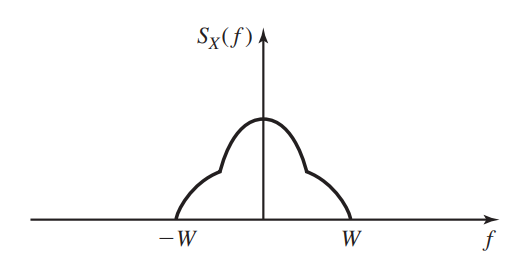
\includegraphics[width=0.8\linewidth]{kekmek1_pic_2.png}
\caption{Ограниченный спектр случайного процесса $X(f)$}
\label{fig:X(f)}
\end{figure}
Типичный пример ограниченного спектра приведен на рис.~\ref{fig:X(f)}.
Теперь мы привели все необходимые понятия, которые необходимы для формулировки следующей теоремы.

\begin{theorem}[Котельникова]
Пусть $X(t)$ стационарный случайный процесс с ограниченным спектром, т.е. $\mathcal{S}_X (f) \equiv 0$ $|f| \geq W $.
Тогда имеет место следующее выражение

{
\centering
\begin{equation}
    E \left| X(t) - \sum\limits_{k=-\infty}^{\infty} X(k T_s) \text{ sinc}(2 W (t-k T_s)) \right| ^ 2 = 0,
\end{equation}
}
где $T_s = \frac{1}{2W}$ определяет интервал прореживания.\\
\end{theorem}
\begin{proof}
Раскроем слагаемое:

\begin{equation*}
	\begin{gathered}
		E \left| X(t) - \sum\limits_{k=-\infty}^{\infty} X(k T_s) \text{ sinc}(2 W (t-k T_s)) \right| ^ 2 = \\
		= R_X(0) - 2\sum\limits_{k=-\infty}^{\infty}R_X(t-k T_s) \text{ sinc}(2 W (t-k T_s)) +\\
		\sum\limits_{k=-\infty}^{\infty}\sum\limits_{l=-\infty}^{\infty} R_X((k-l) T_s)\text{ sinc}(2W(t-k T_s))\text{ sinc}(2W(t-l T_s))
	\end{gathered}
\end{equation*}


В последней строчке приведенного равенства сделаем замену переменных $m = l - k$

{\centering

$\sum\limits_{k=-\infty}^{\infty}\sum\limits_{l=-\infty}^{\infty} R_X((k-l) T_s)\text{ sinc}(2W(t-k T_s))\text{ sinc}(2W(t-l T_s))=$\\
$\sum\limits_{k=-\infty}^{\infty}\sum\limits_{m=-\infty}^{\infty} R_X(-m T_s)\text{ sinc}(2W(t-k T_s))\text{ sinc}(2W(t-k T_s - mT_s)) = $ \\
$\sum\limits_{k=-\infty}^{\infty} \text{ sinc}(2W(t-kT_s)) \sum\limits_{m=-\infty}^{\infty} R_X(mT_s) \text{ sinc}(2W(t-kT_s-mT_s))$
}
Заметим, что последне слагаемое есть разложение в ряд Котельникова функции $R_X(t-kT_s)$, т.е.\\
$\sum\limits_{m=-\infty}^{\infty} R_X(mT_s) \text{ sinc}(2W(t-kT_s-mT_s)) = R_X(t-kT_s)$.

Следовательно, 

{
\centering
$E| X(t) - \sum\limits_{k=-\infty}^{\infty} X(k T_s) \text{ sinc}(2 W (t-k T_s)) | ^ 2 = $\\
$R_X(0) - 2\sum\limits_{k=-\infty}^{\infty}R_X(t-k T_s) \text{ sinc}(2 W (t-k T_s)) +$\\
$\sum\limits_{k=-\infty}^{\infty}R_X(t-k T_s) \text{ sinc}(2 W (t-k T_s))=$\\
$R_X(0) - \sum\limits_{k=-\infty}^{\infty}R_X(t-k T_s) \text{ sinc}(2 W (t-k T_s))$.
}

Нетрудно заметить, что \\ 
$R_X(0) = \sum\limits_{k=-\infty}^{\infty}R_X(t-k T_s) \text{ sinc}(2 W (t-k T_s))$.\\
Следовательно, выполнено необходимое равенство. 

\end{proof}
